\RequirePackage{fixltx2e}
\documentclass{jknotes}
\usepackage{joshkirklin}

\begin{document}

\institution{Cambridge Part III Maths}
\title{The Standard Model}
\lecturer{Christopher Thomas}
\notetaker{Josh Kirklin}
\date{Lent 2016}

\maketitle
\suggestionsspiel
\tableofcontents

\section{Introduction}
\lecture{15/01/16}
The standard model (SM) is the most experimentally successful Quantum Field Theory ever developed. It describes three fundamental forces, each mediated by spin 1 gauge bosons:
\begin{description}
    \item[Electromagnetism]: photon \(\gamma\) (QED)
    \item[Weak interaction]: \(W^\pm\) and \(Z\) bosons
    \item[Strong interaction]: gluons \(g\) (QCD)
\end{description}
The matter in the standard model is present as spin \(\frac{1}{2}\) fermions:
\begin{description}
    \item[Quarks]: \(u\choose d\), \(c\choose s\), \(t\choose b\) and antiparticles. These experience all three interactions.
    \item[Charged leptons]: \(e,\mu,\tau\) and antiparticles. These experience the electromagnetic and weak interactions.
    \item[Neutrinos]: \(\nu_e,\nu_\mu,\nu_\tau\) and antiparticles. These only experience the weak force.
\end{description}
Note that all of these particles appear in three generations with successivly larger masses. We're not absolutely certain why this is the case.

Finally, we have a single scalar spin 0 particle:
\begin{description}
    \item[Higgs boson]: This gives mass to the \(W^\pm\), \(Z\) and the fermions.
\end{description}

The gauge bosons are manifestations of a local gauge symmetry. In the standard model, the gauge group is given by:
\begin{figure}[H]
    \centering
    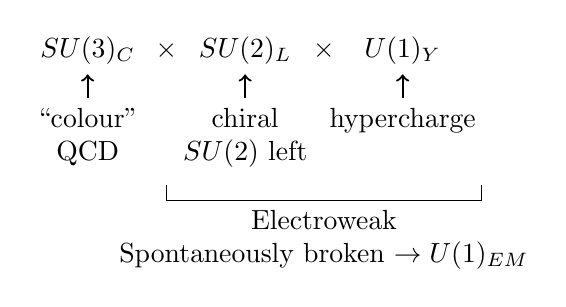
\begin{tikzpicture}
        \node at (0,0) {\(SU(3)_C\)};
        \node at (1,0) {\(\times\)};
        \node at (2,0) {\(SU(2)_L\)};
        \node at (3,0) {\(\times\)};
        \node at (4,0) {\(U(1)_Y\)};
        \draw[<-, thick] (0,-0.3) -- (0,-0.6) node[below, align=center] {``colour''\\QCD};
        \draw[<-, thick] (2,-0.3) -- (2,-0.6) node[below, align=center] {chiral \\\(SU(2)\) left};
        \draw[<-, thick] (4,-0.3) -- (4,-0.6) node[below, align=center] {hypercharge};
        \draw(1,-1.7) -- (1,-1.9) -- (5,-1.9) -- (5,-1.7);
        \node[below,align=center] at (3,-1.9) {Electroweak\\Spontaneously broken \(\rightarrow U(1)_{EM}\)};
    \end{tikzpicture}
\end{figure}

In this course we will take the conventions:
\begin{equation}
    \eta=\eta_s=\eta'=\eta_z=\eta_\theta=\eta_\gamma=\eta_e=+1
\end{equation}
The meanings of these symbols will hopefully become clear.

The course will follow the following general outline:
\begin{itemize}
    \item Symmetries (chiral, gauge, discrete)
    \item Spontaneous symmetry breaking
    \item Electroweak interactions
    \item QCD
    \item Effective field theories
\end{itemize}

\section{Chiral and Gauge symmetries}
To begin, we will review some concepts and set some notation and conventions.

\subsection{Chiral symmetry}
Consider a spin \(\frac{1}{2}\) Dirac fermion with spinor field \(\psi\) that satisfies the Dirac equation:
\begin{equation}
    (i\slashed{\partial}-m)\psi \qq{where} \slashed{\partial} = \gamma^\mu\partial_\mu
\end{equation}
The adjoint \(\overline{\psi}\) satisfies:
\begin{equation}
    \overline{\psi}(i\overleftarrow{\slashed{\partial}}+m)=0 \quad \text{where } \overleftarrow{\partial} \text{ acts to the left.}
\end{equation}
The Dirac matrices \(\gamma^\mu\) satisfy \(\{\gamma^\mu,\gamma^\nu\}=2g^{\mu\nu}\identity\), where \(g_{\mu\nu}=\operatorname{diag}(1,-1,-1,-1)\) is the Minkowski metric. We also define \(\gamma^5=-i\gamma^0\gamma^1\gamma^2\gamma^3\), from which we can deduce \(\left( \gamma^5 \right)^2=1\) and \(\{\gamma^5,\gamma^\mu\}=0\).

The chiral (or Weyl) representation is given by:
\begin{equation}
    \gamma^0 = 
    \begin{pmatrix}
        0 & \identity \\
        \identity & 0
    \end{pmatrix}, \quad
    \gamma^i =
    \begin{pmatrix}
        0 & \sigma^i \\
        -\sigma^i & 0
    \end{pmatrix}, \quad
    \gamma^5 = 
    \begin{pmatrix}
        \identity & 0 \\
        0 & -\identity
    \end{pmatrix}
\end{equation}
where the \(\sigma^i\) are the Pauli matrices.

It is useful to consider the massless Dirac equation \(\slashed{\partial}\psi=0\). We have \(\slashed{\partial}\gamma^5\psi=0\). We can define the projection operators \(P_{L,R} =\frac{1}{2}(1\pm\gamma^5)\), and define \(\psi_{L,R} = P_{L,R}\psi\), from which we can deduce \(\overline{\psi}_{L,R}=\overline{\psi}P_{R,L}\). It is easy to verify that these are projection operators:
\begin{equation}
    P_{L,R}^2=P_{L,R}, \quad P_LP_R=P_RP_L=0, \quad P_L+P_R=1
\end{equation}
In the chiral representation:
\begin{equation}
    P_L = 
    \begin{pmatrix}
        0 & 0 \\
        0 & \identity
    \end{pmatrix}, \quad
    P_R = 
    \begin{pmatrix}
        \identity & 0 \\
        0 & 0
    \end{pmatrix}
\end{equation}
So we can see that in the chiral representation, \(\psi_{L,R}\) only contain respective the lower or upper two components of the spinor degrees of freedom. Also, \(\gamma^5\psi_{L,R}=\pm\psi_{L,R}\), so \(\psi_{L,R}\) have definite chirality, by which we mean they are eigenvectors of \(\gamma^5\).

The massless Dirac equation has \(U(1)_L\times U(1)_R\) chiral symmetry:
\begin{equation}
    \psi_L\rightarrow e^{i\alpha_L}\psi_L,\quad \psi_R\rightarrow e^{i\alpha_R}\psi_R
\end{equation}
\begin{equation}
    \overline{\psi}_{L,R} \rightarrow \overline{\psi}_{L,R} e^{-i\alpha_{L,R}}
\end{equation}

Consider the Dirac Lagrangian where we now include mass:
\begin{align}
    \mathcal{L} &= \overline{\psi}(i\slashed{\partial}-m)\psi\\
    &= \overline{\psi}_Li\slashed{\partial}\psi_L
    + \overline{\psi}_Ri\slashed{\partial}\psi_R
    - m (\overline{\psi}_R\psi_L + \overline{\psi}_L\psi_R )
\end{align}
We see that the kinetic term is invariant under a chiral left and right transformation, but the mass term breaks this symmetry explicitly. It converts it into a vector symmetry. We require \(\alpha_L=\alpha_R\), so:
\begin{equation}
    U(1)_L\times U(1)_R \rightarrow U(1)_V
\end{equation}

\end{document}
